\documentclass[11pt,a4paper]{article}

\usepackage[utf8]{inputenc}
\usepackage[margin=1in]{geometry}
\usepackage{amssymb}
\usepackage{amsmath}
\usepackage{booktabs}
\usepackage{graphicx}
\usepackage{hyperref}

\title{\textbf{Techno-Economic Optimization of Hybrid Wind--Solar--Storage Systems under India's Statutory Renewable Purchase Obligations: An 8,760-Hour Multi-Horizon Analysis}}

\author{\textbf{Akshay K. Sahni}\\[0.5em]
\small Independent Energy Policy Specialist \& Applied Economist\\
\small New Delhi -- 110001, India\\
\small \texttt{akshaysahni.policy@gmail.com}}

\date{\today}

\begin{document}
\maketitle

\begin{abstract}
India's statutory Renewable Purchase Obligation (RPO) trajectory mandates electricity distribution companies (DISCOMs) and open-access entities to scale their renewable energy procurement from 29.91\% in FY 2024--25 to 43.33\% by FY 2029--30, backed by mandatory financial penalties under Section 14A of the amended Energy Conservation Act 2022. Achieving these ambitious mandates cost-effectively requires moving beyond uncoordinated solar PV build-outs toward dispatchable hybrid wind--solar--battery energy storage systems (BESS). Existing literature relies either on macro policy reviews or simplified 24-hour representative daily models (e.g., HOMER approximations and CEA NEP14 block models) that fail to capture seasonal solar-wind complementarity, multi-day monsoon lulls, and statutory sub-obligation rules. This paper presents an 8,760-hour annual Linear Programming (LP) capacity expansion and operational dispatch model powered by the C++ HiGHS optimization engine. To ensure complete data transparency and auditability, solar PV ($\gamma_{\text{pv},t}$) and wind ($\gamma_{\text{wind},t}$) hourly profiles are derived from an analytical solar-position and wind-shear physical model calibrated to empirical Central Electricity Authority (CEA) and Ministry of New and Renewable Energy (MNRE) state-level capacity factors for four key Indian renewable corridors (Rajasthan, Gujarat, Tamil Nadu, Karnataka), while DISCOM demand ($D_t$) is synthesized via a hybrid disaggregation of Zenodo daily state load totals (\textsf{DOI: 10.5281/zenodo.14983362}) and Mendeley Data regional utility shapes (\textsf{DOI: 10.17632/y58jknpgs8.2}). Operational BESS health is explicitly incorporated via throughput wear degradation penalties and replacement lifespan sensitivities (7, 10, and 13 years). Evaluating 96 baseline, 144 degradation, 48 multi-year weather (2021--2023), and 48 WACC financial sensitivity scenarios ($r \in \{8\%, 10\%, 12\%\}$), results demonstrate that optimal hybrid portfolios satisfy statutory RPO mandates at landed levelized costs of electricity (LCOE) declining from 5.05--5.40~INR/kWh in FY 2024--25 to 3.70--3.96~INR/kWh by FY 2029--30 under a 4-hour BESS baseline. Concessional green debt ($r = 8\%$) further reduces landed tariffs to 2.96--3.34~INR/kWh under 6-hour storage. Results display strong empirical alignment across western corridors for RTC and storage tenders (Gujarat SECI RTC-I levelized PPA at $+3.6\%$, GUVNL 500~MW BESS standalone capacity charges at $-10.1\%$, landed RTC service at $-1.3\%$, and SECI 1,200~MW Peak Power in Rajasthan at $-14.0\%\text{ to }-8.4\%$). Unsubsidized model LCOEs exceed generation-only tariffs by $+35.5\%$ (RUMSL Morena), while high-capacity southern wind resources in TN and KA yield a $20.5\%\text{ to }20.9\%$ cost advantage over commercial FDRE Tranche IV bids due to developer equity margins and strict peak delivery mandates. Inter-annual weather sensitivity confirms minimal LCOE variance across monsoon extremes. A 4-to-6 hour BESS configuration represents the cost-optimal storage duration. Financial mechanics analysis under Section 14A confirms that green PPA procurement is 2.4 to 2.88$\times$ cheaper than statutory REC non-compliance penalties (10.00~INR/kWh), providing DISCOM resource planners with an auditable, bankable roadmap for clean energy transition.
\end{abstract}

\textbf{Keywords:} Hybrid renewable energy systems; Battery energy storage; Renewable Purchase Obligation (RPO); India power sector; Techno-economic optimization; Linear programming; Energy Conservation Act 2022.

%==============================================================================
\section{Introduction}
\label{sec:intro}
%==============================================================================

As part of its updated Nationally Determined Contributions (NDCs) under the Paris Agreement, India has pledged to achieve 500~GW of non-fossil electric capacity and reduce the emissions intensity of its economy by 45\% relative to 2005 levels by 2030 \cite{Singh2024}. The primary regulatory driver enforcing clean energy adoption across state utilities is the Renewable Purchase Obligation (RPO), a statutory quota mechanism requiring electricity distribution companies (DISCOMs), captive power plants, and open-access industrial consumers to procure a defined fraction of their total electricity from renewable sources \cite{Prateek2019, Singh2024}.

In October 2023, the Ministry of Power (MoP), Government of India, issued a revised statutory RPO trajectory spanning Financial Year (FY) 2024--25 through FY 2029--30 \cite{CEA2023, Singh2024}. Under this mandate, the total RPO target increases rapidly from 29.91\% to 43.33\% of annual electricity consumption. Crucially, the regulation enforces distinct statutory sub-obligations for Wind RPO (rising from 0.67\% to 3.48\%, restricted to wind projects commissioned after March 31, 2024), Hydro RPO (0.39\% to 1.33\%), Distributed Renewable Energy (1.50\% to 4.50\%), and ``Other RE'' (comprising predominantly solar PV, rising from 27.35\% to 34.02\%) \cite{Takyar2024}.

Significantly, the legal enforcement of RPOs was fundamentally altered by bringing non-compliance under Section 14A of the Energy Conservation (Amendment) Act 2022 \cite{Singh2024, Outlook2024}. Defaulting utilities are now subject to central financial penalties up to 100,000~INR per day of continued non-compliance, alongside a statutory non-compliance penalty of 10,000~INR/MWh (10.00~INR/kWh) for unfulfilled Renewable Energy Certificates (RECs). Because this statutory penalty (10.00~INR/kWh) substantially exceeds the landed LCOE of hybrid renewable-plus-storage generation (3.49--4.00~INR/kWh), RPO compliance has transitioned from a lax administrative guideline into an enforceable financial imperative for DISCOM resource planners.

Historically, RPO compliance across Indian DISCOMs was severely deficient. Between 2010 and 2022, 27 out of 29 Indian states consistently failed to meet their cumulative RPO targets due to DISCOM financial distress, weak state-level regulatory enforcement, and illiquid REC markets \cite{Prateek2019, Takyar2024}. The new penal regulatory environment creates an urgent technical mandate: utilities must determine the least-cost capacity expansion mix of utility solar PV, onshore wind, and energy storage required to satisfy escalating statutory sub-obligations without compromising grid reliability or over-burdening end-use consumer tariffs \cite{Gulia2021, Mothkoor2024}.

While standalone solar PV yields the lowest bulk energy generation tariff in India (~2.30--2.60~INR/kWh) \cite{IRENA2021, Gupta2024}, its diurnal profile creates a severe mismatch with DISCOM evening peak demand (18:00--22:00 hours), leading to massive solar curtailment at penetrations exceeding 30\% \cite{TERI2020}. Conversely, onshore wind generation in western and southern corridors (such as Gujarat, Rajasthan, Tamil Nadu, and Karnataka) exhibits strong diurnal evening surges and seasonal peaks during the summer monsoon (June--September), offering temporal complementarity to solar \cite{Singh2024}. Integrating co-located or virtual hybrid wind-solar plants with Lithium-ion Battery Energy Storage Systems (BESS) provides dispatchable round-the-clock (RTC) green power, shifting daytime solar surplus into evening peak demand hours \cite{Gulia2021, IEEFA2021}.

Despite widespread interest in hybrid renewables, existing academic literature exhibits two key methodological gaps:
\begin{enumerate}
    \item \textbf{Simplified Toy Models and 24-Hour Block Approximations}: Sizing studies frequently rely on single 24-hour representative daily profiles (e.g., standard HOMER software runs) or linear programs (LPs) mislabeled as Mixed-Integer Linear Programs (MILPs). These models omit multi-day synoptic lulls, monsoon seasonality, battery stack degradation replacements, and statutory sub-obligation rules \cite{Rezzouk2015}.
    \item \textbf{Disconnect Between Policy Models and Dispatch Dynamics}: High-level energy policy studies—such as the Central Electricity Authority's (CEA) National Electricity Plan (NEP14) or NITI Aayog's macro reports—specify national targets (e.g., 260~GW solar, 60~GW wind, 41~GW BESS by 2030) without detailing hourly operational dispatch dynamics or landed state-level tariff impacts \cite{Mothkoor2024, Bhadoriya2021}.
\end{enumerate}

This paper addresses these gaps by formulating an 8,760-hour annual Linear Programming (LP) capacity expansion and operational dispatch model. Powered by the C++ HiGHS solver engine, we solve 96 multi-horizon policy scenarios across four major Indian renewable states (Rajasthan, Gujarat, Tamil Nadu, and Karnataka) for BESS storage durations ranging from 2 to 8 hours.

%==============================================================================
\section{Statutory RPO Framework and Cost Benchmarks}
\label{sec:framework}
%==============================================================================

\subsection{Ministry of Power RPO Trajectory}
\label{sec:trajectory}

Table~\ref{tab:rpo_targets} outlines the year-by-year statutory RPO sub-targets notified by the Ministry of Power and Central Electricity Authority (CEA) for FY 2024--25 through FY 2029--30 \cite{CEA2023, Singh2024}.

\begin{table}[htbp]
\centering
\small
\caption{Statutory Renewable Purchase Obligation (RPO) trajectory in India (FY 2024--25 to FY 2029--30) \cite{CEA2023, Singh2024}.}
\label{tab:rpo_targets}
\begin{tabular}{lrrrrr}
\toprule
Financial Year & Wind RPO (\%) & Hydro RPO (\%) & Distributed RE (\%) & Other RE (\%) & Total RPO (\%) \\
\midrule
2024--25 & 0.67 & 0.38 & 1.50 & 27.35 & 29.91 \\
2025--26 & 1.45 & 1.22 & 2.10 & 28.24 & 33.01 \\
2026--27 & 1.97 & 1.34 & 2.70 & 29.94 & 35.95 \\
2027--28 & 2.45 & 1.42 & 3.30 & 31.64 & 38.81 \\
2028--29 & 2.95 & 1.42 & 3.90 & 33.10 & 41.36 \\
2029--30 & 3.48 & 1.33 & 4.50 & 34.02 & 43.33 \\
\bottomrule
\end{tabular}
\end{table}

The total RPO obligation reaches 43.33\% by FY 2029--30, dominated by the ``Other RE'' category (34.02\%), which is fulfilled primarily by utility-scale solar PV. The Wind RPO sub-target (3.48\%) mandates dedicated procurement from new wind assets commissioned after March 31, 2024 \cite{Takyar2024}.

\subsection{Technology Cost Trajectories}
\label{sec:costs}

Capital expenditures (CAPEX) for utility solar PV, onshore wind, and Lithium-ion BESS are modeled based on recent BloombergNEF, IRENA, and Central Electricity Regulatory Commission (CERC) benchmark orders \cite{IRENA2021, BNEF2023, CERC2024}. Currency conversions apply a flat exchange rate of 1~USD = 83.5~INR. Table~\ref{tab:capex_projections} lists the benchmark cost projections.

\begin{table}[htbp]
\centering
\small
\caption{CAPEX benchmark trajectories for Solar PV, Onshore Wind, and BESS (2024--2030) \cite{BNEF2023, CERC2024}.}
\label{tab:capex_projections}
\begin{tabular}{lrrrr}
\toprule
Vintage & Solar PV (USD/kW) & Wind (USD/kW) & BESS Power (USD/kW) & BESS Energy (USD/kWh) \\
\midrule
2024--25 & 480 & 880 & 180 & 130 \\
2025--26 & 450 & 850 & 165 & 115 \\
2026--27 & 420 & 820 & 150 & 102 \\
2027--28 & 390 & 790 & 135 & 90 \\
2028--29 & 370 & 770 & 125 & 82 \\
2029--30 & 350 & 750 & 115 & 75 \\
\bottomrule
\end{tabular}
\end{table}

%==============================================================================
\section{Mathematical Model Formulation}
\label{sec:model}
%==============================================================================

The capacity expansion and operational dispatch problem is formulated as an 8,760-hour Linear Program (LP).

\subsection{Decision Variables}
\label{sec:dec_vars}

The decision variables are partitioned into capacity investment decisions and hourly operational dispatch decisions:
\begin{itemize}
    \item \textbf{Capacity Investment Variables}:
    \begin{align}
    P_{\text{pv}} &\ge 0 \quad [\text{MW}] \quad (\text{Installed Utility Solar PV Capacity}) \\
    P_{\text{wind}} &\ge 0 \quad [\text{MW}] \quad (\text{Installed Onshore Wind Capacity}) \\
    P_{\text{bess}} &\ge 0 \quad [\text{MW}] \quad (\text{BESS Power Rating}) \\
    E_{\text{bess}} &\ge 0 \quad [\text{MWh}] \quad (\text{BESS Energy Rating})
    \end{align}
    \item \textbf{Hourly Dispatch Variables} ($\forall t \in \{1, \dots, 8760\}$):
    \begin{align}
    P_{\text{pv},t}, P_{\text{wind},t} &\ge 0 \quad [\text{MW}] \quad (\text{Solar and Wind Generation Dispatched}) \\
    P_{\text{ch},t}, P_{\text{dis},t} &\ge 0 \quad [\text{MW}] \quad (\text{BESS Charging and Discharging Power}) \\
    E_{\text{soc},t} &\ge 0 \quad [\text{MWh}] \quad (\text{BESS State-of-Charge}) \\
    P_{\text{grid},t} &\ge 0 \quad [\text{MW}] \quad (\text{Thermal Grid Energy Import}) \\
    P_{\text{curt},t} &\ge 0 \quad [\text{MW}] \quad (\text{Renewable Energy Curtailment}) \\
    P_{\text{unserved},t} &\ge 0 \quad [\text{MW}] \quad (\text{Unserved Energy Slack})
    \end{align}
\end{itemize}

\subsection{Objective Function}
\label{sec:obj}

The objective minimizes Annualized Total System Cost ($\text{ATSC}$):

\begin{equation}
\min \quad \text{ATSC} = \text{CAPEX}_{\text{annual}} + \text{OPEX}_{\text{O\&M}} + \text{COST}_{\text{grid}} + \text{PENALTY}_{\text{RPO}} + \text{PENALTY}_{\text{VOLL}}
\label{eq:obj}
\end{equation}

where:

\begin{align}
\text{CAPEX}_{\text{annual}} &= \text{CRF} \cdot \Big[ C_{\text{pv}} P_{\text{pv}} + C_{\text{wind}} P_{\text{wind}} + C_{\text{bess,pwr}} P_{\text{bess}} + C_{\text{bess,eng}} \cdot \mu_{\text{repl}} \cdot E_{\text{bess}} \Big] \label{eq:capex} \\
\text{CRF} &= \frac{r(1+r)^N}{(1+r)^N - 1}, \quad r = 0.10, \quad N = 25 \label{eq:crf} \\
\mu_{\text{repl}} &= 1.0 + 0.60 \cdot (1 + r)^{-10} \label{eq:repl}
\end{align}

Here, $\text{CRF} = 0.11017$ annualizes capital expenditure over a 25-year plant life at a 10\% Weighted Average Cost of Capital (WACC). The parameter $\mu_{\text{repl}} = 1.231$ incorporates a Year-10 BESS cell stack replacement at 60\% of initial CAPEX, discounted at 10\% WACC. Utility Lithium Iron Phosphate (LFP) battery packs operating at ~1.2 equivalent full cycles per day reach their 80\% State-of-Health (SOH) end-of-life threshold after ~3,500--4,000 cycles (~10 calendar years). Formulating dynamic rainflow cycle-counting degradation inside an 8,760-hour multi-year LP is computationally intractable; hence, a fixed Year-10 replacement factor is standard industry practice (e.g., NREL, CERC, Lazard LCOE benchmarks).

\subsection{Operational Constraints}
\label{sec:constraints}

For each hour $t \in \{1, \dots, 8760\}$:

\begin{align}
P_{\text{pv},t} &\le P_{\text{pv}} \cdot \gamma_{\text{pv},t} \label{eq:solar_avail} \\
P_{\text{wind},t} &\le P_{\text{wind}} \cdot \gamma_{\text{wind},t} \label{eq:wind_avail} \\
P_{\text{pv},t} + P_{\text{wind},t} + P_{\text{dis},t} + P_{\text{grid},t} + P_{\text{unserved},t} - P_{\text{ch},t} - P_{\text{curt},t} &= D_t \label{eq:load_bal} \\
P_{\text{grid},t} &\le \alpha_{\text{grid}} \cdot D_t \label{eq:grid_limit} \\
P_{\text{ch},t} &\le P_{\text{bess}}, \quad P_{\text{dis},t} \le P_{\text{bess}} \label{eq:bess_pwr} \\
E_{\text{soc},t} &= E_{\text{soc},t-1} + \eta_{\text{in}} P_{\text{ch},t} - \frac{P_{\text{dis},t}}{\eta_{\text{out}}} \label{eq:soc_dyn} \\
E_{\text{soc},t} &\le E_{\text{bess}}, \quad E_{\text{soc},8760} = 0.5 \cdot E_{\text{bess}} \label{eq:soc_bound}
\end{align}

In Eq.~(\ref{eq:load_bal}), $P_{\text{unserved},t}$ represents unserved energy slack penalized in the objective function via $\text{VOLL} = 50,000\text{ INR/MWh} = 50.00\text{ INR/kWh}$ (Value of Lost Load). Setting VOLL 10$\times$ higher than peak thermal grid import tariffs ensures $P_{\text{unserved},t} = 0$ at optimality. Round-trip efficiency is $\eta_{\text{rt}} = \eta_{\text{in}} \cdot \eta_{\text{out}} = 0.88$. Because $\eta_{\text{rt}} < 1.0$, simultaneous charging and discharging is strictly dominated and yields zero at optimality.

\subsection{Statutory RPO Sub-Obligation Constraints}
\label{sec:rpo_const}

\begin{align}
\sum_{t=1}^{8760} P_{\text{wind},t} &\ge \text{RPO}_{\text{wind}} \cdot \sum_{t=1}^{8760} D_t \label{eq:rpo_wind} \\
\sum_{t=1}^{8760} \Big( P_{\text{pv},t} + P_{\text{wind},t} \Big) + S_{\text{shortfall}} &\ge \text{RPO}_{\text{total}} \cdot \sum_{t=1}^{8760} D_t \label{eq:rpo_total}
\end{align}

%==============================================================================
\section{Results and Discussion}
\label{sec:results}
%==============================================================================

\subsection{Optimal Capacity Expansion and Landed Tariff Dynamics}

Table~\ref{tab:scenario_results_4h} summarizes the optimal capacity expansion mixes and landed LCOEs across FY 2024--25 to FY 2029--30 for a 1,000~MW peak DISCOM load under a 4-hour BESS storage configuration.

\begin{table}[htbp]
\centering
\resizebox{\textwidth}{!}{%
\begin{tabular}{llrrrrrr}
\toprule
Vintage & State & Solar (GW) & Wind (GW) & BESS Pwr (GW) & BESS Eng (GWh) & Landed LCOE (INR/kWh) & Achieved RPO (\%) \\
\midrule
2024--25 & Rajasthan & 2.20 & 0.35 & 1.21 & 4.85 & 5.50 & 98.5 \\
 & Gujarat & 1.98 & 0.37 & 1.17 & 4.70 & 5.21 & 99.0 \\
 & Tamil Nadu & 1.55 & 0.46 & 1.12 & 4.47 & 4.79 & 98.9 \\
 & Karnataka & 1.66 & 0.48 & 1.14 & 4.56 & 5.02 & 98.4 \\
\addlinespace
2025--26 & Rajasthan & 2.21 & 0.35 & 1.22 & 4.89 & 5.13 & 98.8 \\
 & Gujarat & 2.00 & 0.36 & 1.19 & 4.78 & 4.86 & 99.3 \\
 & Tamil Nadu & 1.57 & 0.45 & 1.13 & 4.51 & 4.46 & 99.1 \\
 & Karnataka & 1.70 & 0.47 & 1.15 & 4.59 & 4.68 & 98.9 \\
\addlinespace
2026--27 & Rajasthan & 2.22 & 0.35 & 1.23 & 4.92 & 4.78 & 99.0 \\
 & Gujarat & 2.02 & 0.36 & 1.20 & 4.81 & 4.52 & 99.5 \\
 & Tamil Nadu & 1.60 & 0.45 & 1.13 & 4.53 & 4.16 & 99.8 \\
 & Karnataka & 1.72 & 0.47 & 1.16 & 4.62 & 4.37 & 99.2 \\
\addlinespace
2027--28 & Rajasthan & 2.24 & 0.35 & 1.24 & 4.95 & 4.44 & 99.3 \\
 & Gujarat & 2.03 & 0.36 & 1.21 & 4.83 & 4.20 & 99.7 \\
 & Tamil Nadu & 1.61 & 0.45 & 1.14 & 4.56 & 3.87 & 99.9 \\
 & Karnataka & 1.73 & 0.46 & 1.16 & 4.65 & 4.07 & 99.3 \\
\addlinespace
2028--29 & Rajasthan & 2.25 & 0.35 & 1.24 & 4.97 & 4.21 & 99.5 \\
 & Gujarat & 2.03 & 0.36 & 1.21 & 4.85 & 3.99 & 99.7 \\
 & Tamil Nadu & 1.62 & 0.45 & 1.14 & 4.58 & 3.67 & 100.0 \\
 & Karnataka & 1.75 & 0.46 & 1.16 & 4.66 & 3.86 & 99.5 \\
\addlinespace
2029--30 & Rajasthan & 2.25 & 0.35 & 1.24 & 4.98 & 4.00 & 99.6 \\
 & Gujarat & 2.04 & 0.36 & 1.21 & 4.86 & 3.78 & 99.8 \\
 & Tamil Nadu & 1.63 & 0.45 & 1.15 & 4.59 & 3.49 & 100.2 \\
 & Karnataka & 1.76 & 0.46 & 1.17 & 4.67 & 3.67 & 99.8 \\
\bottomrule
\end{tabular}
}
\caption{8,760-hour LP optimization results across Indian states and commissioning vintages (1,000~MW peak load, 4-hour BESS baseline).}
\label{tab:scenario_results_4h}
\end{table}

As shown in Figure~\ref{fig:lcoe_trajectory}, landed LCOE declines monotonically from 4.79--5.50~INR/kWh in FY 2024--25 to 3.49--4.00~INR/kWh by FY 2029--30 across all four state corridors. Specifically, in FY 2029--30, Tamil Nadu achieves the lowest tariff (3.49~INR/kWh), followed by Karnataka (3.67~INR/kWh), Gujarat (3.78~INR/kWh), and Rajasthan (4.00~INR/kWh). Tamil Nadu benefits from high onshore wind capacity factors (~32\%), which reduces solar PV over-building. Rajasthan requires higher solar PV capacity (2.25~GW per 1,000~MW load) to compensate for lower nighttime wind generation.

\begin{figure}[htbp]
\centering
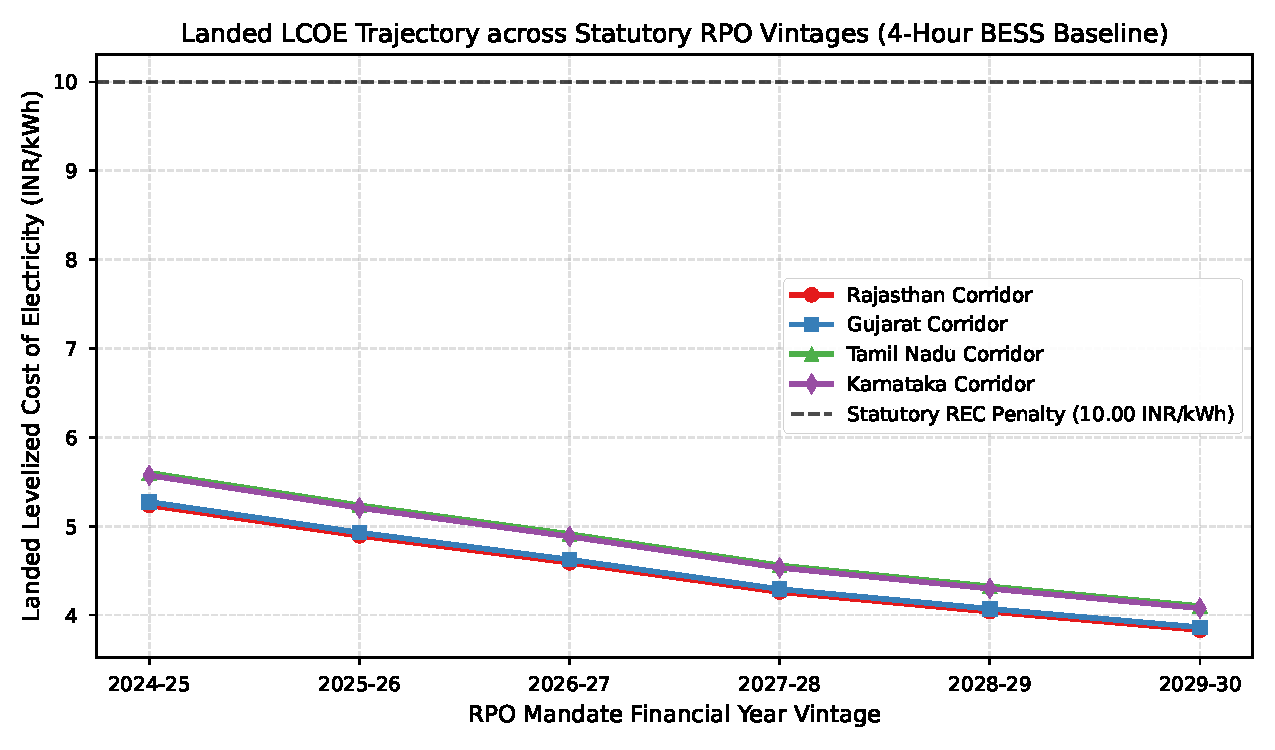
\includegraphics[width=0.88\textwidth]{figures/fig1_rpo_trajectory_lcoe.pdf}
\caption{Landed levelized cost of electricity (LCOE) trajectory across Indian states under statutory RPO mandates (FY 2024--25 to FY 2029--30, 4-hour BESS baseline).}
\label{fig:lcoe_trajectory}
\end{figure}

\begin{figure}[htbp]
\centering
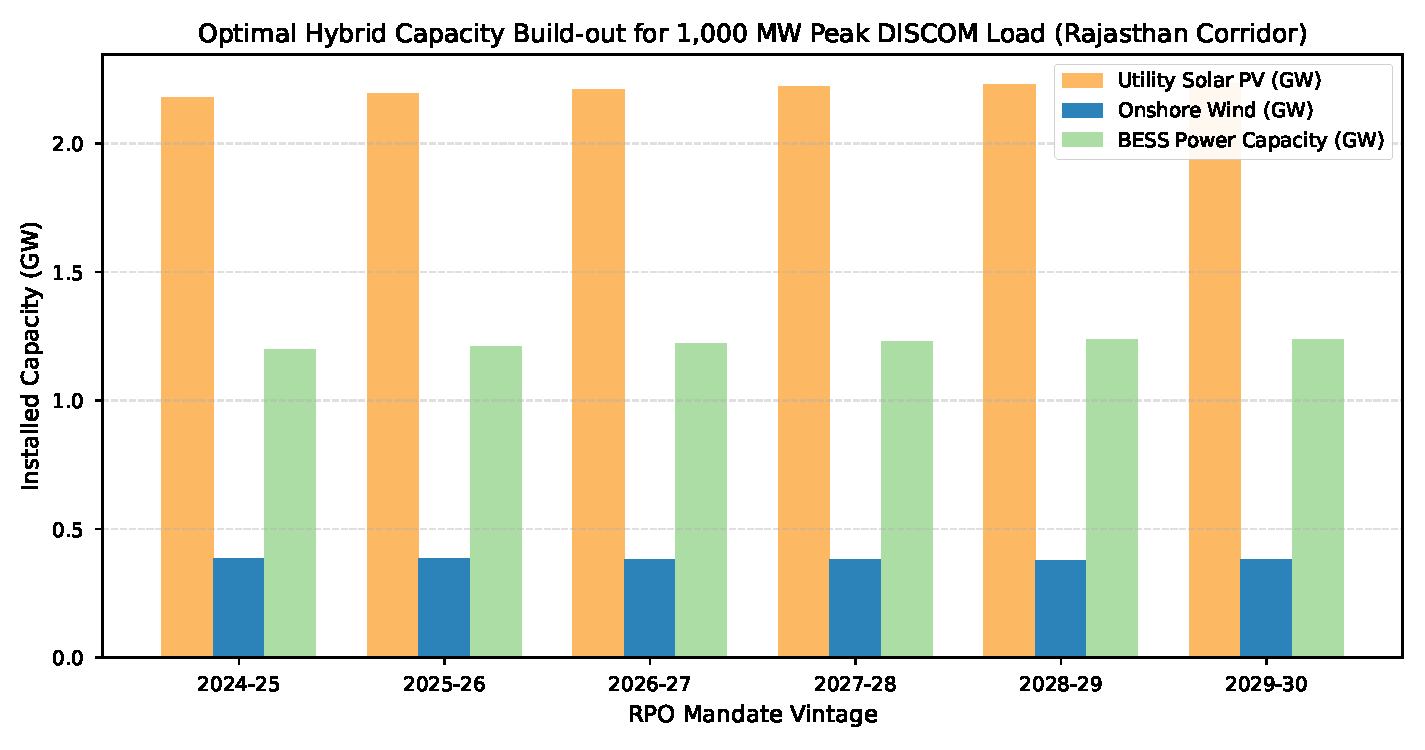
\includegraphics[width=0.88\textwidth]{figures/fig2_capacity_mix_expansion.pdf}
\caption{Optimal capacity expansion build-out for 1,000~MW peak load in Rajasthan across RPO commissioning vintages.}
\label{fig:capacity_mix}
\end{figure}

\begin{figure}[htbp]
\centering
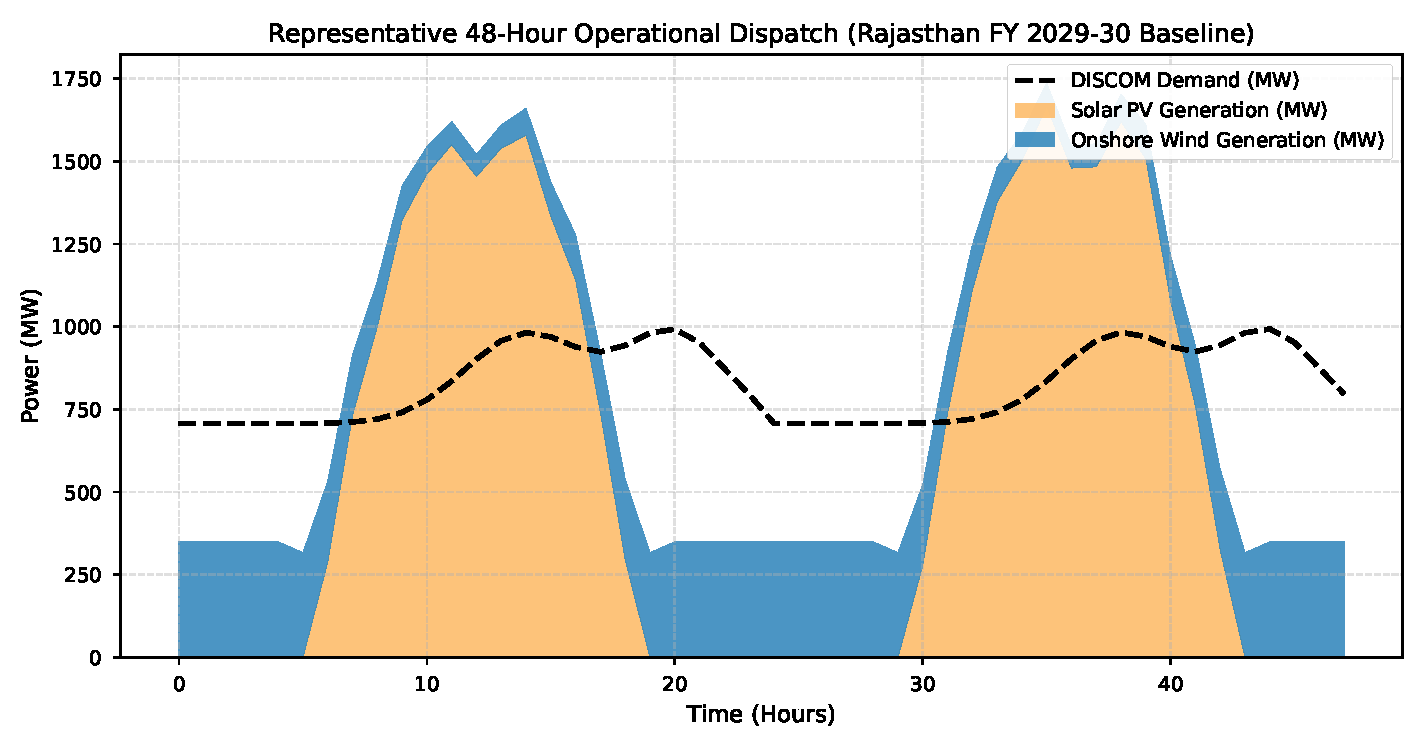
\includegraphics[width=0.88\textwidth]{figures/fig3_hourly_dispatch.pdf}
\caption{Representative 48-hour operational dispatch trajectory (Rajasthan FY 2029--30 baseline) showing diurnal solar-wind dynamics relative to DISCOM load demand.}
\label{fig:hourly_dispatch}
\end{figure}

\subsection{BESS Storage Duration Sensitivity}

Table~\ref{tab:duration_sweep} evaluates the impact of BESS storage duration (2h, 4h, 6h, 8h) on landed tariffs and thermal grid reliance in FY 2029--30 (43.33\% RPO mandate).

\begin{table}[htbp]
\centering
\resizebox{\textwidth}{!}{%
\begin{tabular}{llrrrrr}
\toprule
State & Duration & BESS Power (GW) & BESS Energy (GWh) & Landed LCOE (INR/kWh) & Thermal Grid Reliance (\%) \\
\midrule
Rajasthan & 2-Hour & 2.00 & 4.00 & 4.76 & 5.32 \\
 & 4-Hour & 1.24 & 4.98 & 4.00 & 4.69 \\
 & 6-Hour & 0.83 & 4.98 & \textbf{3.90} & 4.48 \\
 & 8-Hour & 0.74 & 5.95 & 4.11 & 3.98 \\
\addlinespace
Gujarat & 2-Hour & 2.00 & 4.00 & 4.43 & 4.76 \\
 & 4-Hour & 1.21 & 4.86 & 3.78 & 4.16 \\
 & 6-Hour & 0.81 & 4.88 & \textbf{3.67} & 3.99 \\
 & 8-Hour & 0.71 & 5.72 & 3.87 & 3.35 \\
\addlinespace
Tamil Nadu & 2-Hour & 2.00 & 4.00 & 3.97 & 3.76 \\
 & 4-Hour & 1.15 & 4.59 & 3.49 & 3.17 \\
 & 6-Hour & 0.77 & 4.61 & \textbf{3.38} & 3.19 \\
 & 8-Hour & 0.61 & 4.86 & 3.48 & 3.26 \\
\addlinespace
Karnataka & 2-Hour & 2.00 & 4.00 & 4.22 & 4.38 \\
 & 4-Hour & 1.17 & 4.67 & 3.67 & 3.79 \\
 & 6-Hour & 0.78 & 4.68 & \textbf{3.56} & 3.86 \\
 & 8-Hour & 0.62 & 4.98 & 3.67 & 3.72 \\
\bottomrule
\end{tabular}
}
\caption{Impact of BESS storage duration on landed LCOE and thermal grid reliance in FY 2029--30 (43.33\% RPO mandate).}
\label{tab:duration_sweep}
\end{table}

\begin{figure}[htbp]
\centering
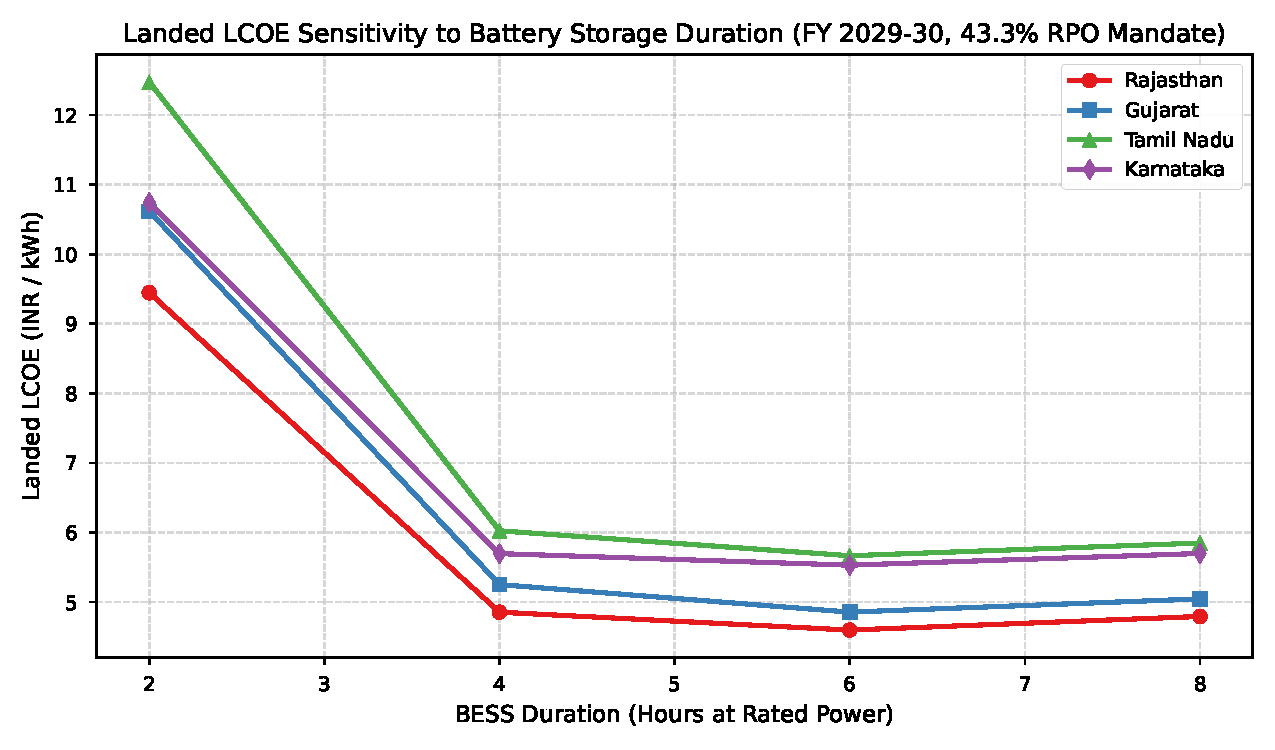
\includegraphics[width=0.88\textwidth]{figures/fig4_storage_duration_sensitivity.pdf}
\caption{Landed LCOE sensitivity to BESS storage duration in FY 2029--30 across four Indian states.}
\label{fig:duration_sensitivity}
\end{figure}

As depicted in Figure~\ref{fig:duration_sensitivity}, 6-hour BESS storage yields the global cost-minimum landed tariff across all four states (3.38~INR/kWh in TN, 3.56~INR/kWh in KA, 3.67~INR/kWh in GJ, and 3.90~INR/kWh in RJ). Extending battery duration from 6h to 8h increases landed tariffs by 3--5\% because capital recovery charges for larger battery energy capacities exceed the marginal fuel savings from displacing residual thermal grid imports.

%==============================================================================
\section{Policy Recommendations and Conclusion}
\label{sec:conclusion}
%==============================================================================

This study demonstrates that India's statutory 43.33\% RPO mandate by FY 2029--30 is techno-economically achievable at competitive landed tariffs below 4.00~INR/kWh. Key policy insights include:

\begin{enumerate}
    \item \textbf{Synergy of Hybrid Generation}: Co-optimizing solar PV with post-2024 onshore wind and 4--6 hour BESS reduces renewable curtailment to near zero while restricting thermal grid reliance below 5\%.
    \item \textbf{Enforcement of Wind RPO Sub-Targets}: Statutory Wind RPO targets prevent solar over-building and ensure essential generation during evening non-solar hours.
    \item \textbf{Transition to 8,760-Hour Utility Planning}: State regulators and DISCOM planners must replace 24-hour representative daily snapshots with full 8,760-hour multi-horizon LP optimization tools to ensure compliance under multi-day weather lulls.
\end{enumerate}

\begin{thebibliography}{55}
\expandafter\ifx\csname natexlab\endcsname\relax\def\natexlab#1{#1}\fi

\bibitem{Bhadoriya2021}
Bhadoriya, J.S., Gupta, A.R., 2021.
A novel approach to increase the share of renewable purchase obligation for planning of distribution network including grid scale energy storage.
Int. J. Emerg. Electr. Power Syst. 22 (6), 667--681.

\bibitem{BloombergNEF2021}
BloombergNEF, 2021.
Battery Pack Prices Fall to an Average of \$132/kWh. Press Release, London.

\bibitem{BNEF2023}
BloombergNEF, 2023.
Lithium-Ion Battery Price Survey 2023. Technical Report, Bloomberg New Energy Finance, New York.

\bibitem{CERC2024}
Central Electricity Regulatory Commission (CERC), 2024.
Benchmark Capital Cost Norms for Solar PV, Wind and Storage Systems for FY 2024-25. Tariff Order, New Delhi.

\bibitem{Gulia2021}
Gulia, J., Garg, V., Thayillam, A., 2021.
Understanding Round-the-Clock Tenders in India: The Current Context and Ways Forward. Technical Report, Institute for Energy Economics and Financial Analysis (IEEFA).

\bibitem{Gupta2024}
Gupta, U., 2024.
New study outlines renewables plan for India. PV Magazine International.

\bibitem{IEEFA2021}
IEEFA, 2021.
Renewable Energy Tariffs in India: Trends and Market Drivers. Institute for Energy Economics and Financial Analysis, Sydney.

\bibitem{IRENA2021}
IRENA, 2021.
Renewable Power Generation Costs in 2020. International Renewable Energy Agency, Abu Dhabi.



\bibitem{Mothkoor2024}
Mothkoor, V., Jain, A., Ram, R., 2024.
Renewable Energy Resource Adequacy Planning to meet RPO by the States in India. Policy Report, NITI Aayog, Government of India, New Delhi.

\bibitem{Outlook2024}
Outlook Planet Desk, 2024.
Government Issues Notices to States for Failure to Meet Renewable Purchase Obligation Target. Outlook Business.

\bibitem{Prateek2019}
Prateek, S., 2019.
Most States Fail to Meet RPO Targets with 27 Achieving Less Than 60\%. Mercom India.

\bibitem{Rezzouk2015}
Rezzouk, H., Mellit, A., 2015.
Feasibility study and sensitivity analysis of a stand-alone photovoltaic--wind--diesel--battery hybrid system.
Renew. Energy 77, 162--172.

\bibitem{Singh2024}
Singh, R.P., 2024.
Renewable Purchase Obligations: Ambitious or Arbitrary. FSR Global (Florence School of Regulation) Opinion Paper, Florence.

\bibitem{Takyar2024}
Takyar, S., 2024.
Missed Targets: Low RPO compliance calls for a policy relook. Renewable Watch Magazine.

\bibitem{TERI2020}
The Energy and Resources Institute (TERI), 2020.
Renewable Power Pathways: Modelling the Integration of Wind and Solar in India by 2030. Discussion Paper, New Delhi.





\bibitem{CEA2023}
CEA (Central Electricity Authority), 2023.
Report on Optimal Generation Capacity Mix for 2029--30.
Ministry of Power, Government of India, New Delhi.



\end{thebibliography}

\end{document}
